\documentclass[11pt,letterpaper,journal]{IEEEtran}
\usepackage[utf8]{inputenc}
\usepackage{graphicx}
\usepackage[numbers]{natbib}
\usepackage{hyperref}
\usepackage{grffile}
\usepackage{todo}
\usepackage{subcaption}
\usepackage{caption}
\usepackage{wrapfig}
% \usepackage[margin=0.5in]{geometry}

\DeclareGraphicsExtensions{.pdf,.png,.jpg}
\graphicspath{ {./img/} }
\newsavebox{\largestimage}

\begin{document}

\markboth{CSCI3341 Final Project Report}{}

\title{Whole-artist imitation with convolutional neural networks}
\author{\IEEEauthorblockN{Jesse Mu\IEEEauthorrefmark{1}\IEEEauthorrefmark{3},
Andrew Francl\IEEEauthorrefmark{2}\IEEEauthorrefmark{3}}\\
\IEEEauthorblockA{Boston College \\
  Email: \IEEEauthorrefmark{1}muj@bc.edu,
  \IEEEauthorrefmark{2}francl@bc.edu\\
  \IEEEauthorrefmark{3}\emph{Both authors contributed equally}
}}
\maketitle

\begin{abstract}
We implemented a machine learning algorithm described in a recent paper by
Gatys et al \cite{gatys15}. The algorithm in the paper describes an
optimization procedure using a convolutional neural network that enables a
given photograph to be recreated in the style of other photographs, notably
paintings. Specifically, the algorithm is able to take a painting and learn its
stylistic composition rather than its content, then apply this stylistic
information to create a new version of the image that stylistically matches the
original painting. We create a Python command-line tool, \texttt{art.py}, that
wraps around the algorithm and extends its functionality by enabling
color-invariant replication according to a randomly selected work in an
artist's oeuvre, increasing the versatility and authenticity of the algorithm's
results. We also discuss possible extesions to the algorithm that will allow
for even more realistic ``whole-artist'' replication in this vein.
\end{abstract}

\section{Introduction}

Recently, a set of algorithms and methods in a field of computer science called
deep learning has seen significant success in various machine learning tasks,
far surpassing the performance of other statistical methods \cite{lecun2015}.
These systems, known as ``neural networks'' (NNs) (Figure~\ref{fig:nn}) and
loosely inspired by biological, connectivist models of human neuroanatomy, have
been especially successful in computer vision, where a specific set of networks
called ``convolutional neural networks'' (CNNs) mimic the complex perceptual
systems in the human visual cortex \cite{riesenhuber99}. In particular, hidden
layers of deep CNNs are capable of learning hierarchical representations of
objects by first analyzing individual pixels and then combining these pixels to
make increasingly complex features (Figure~\ref{fig:comparison}).

\begin{figure}[h]
  \centering
  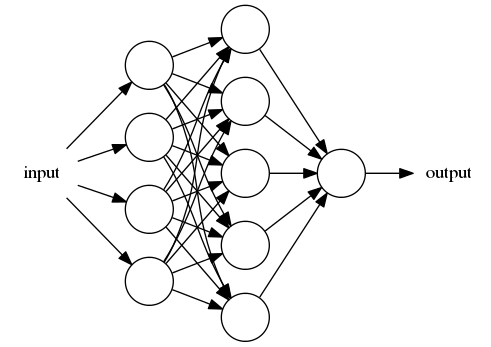
\includegraphics[width=0.8\linewidth]{nn.dot.png}
  \caption{Basic neural network structure, consisting of 4 input neurons
  (left), 5 hidden neurons (center), and one output neuron (right). Computation
  at each neuron is a relatively simple function e.g.\ sigmod activation
  function; numerous combinations of simple functions like these enable complex,
nonlinear output.}
  \label{fig:nn}
\end{figure}

\begin{figure*}[t!]
  \centering

    \begin{subfigure}[t]{0.5\textwidth}
        \centering
        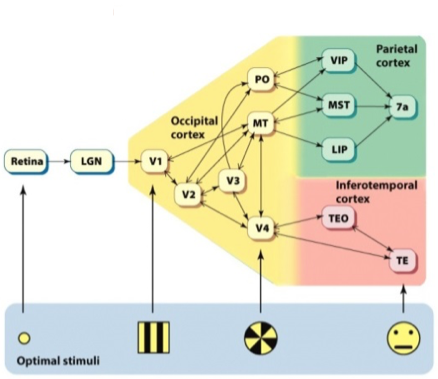
\includegraphics[height=6cm]{vc.png}
        \caption{Visual Cortex}
        \label{fig:vc}
    \end{subfigure}%
    ~
    \begin{subfigure}[t]{0.5\textwidth}
        \centering
        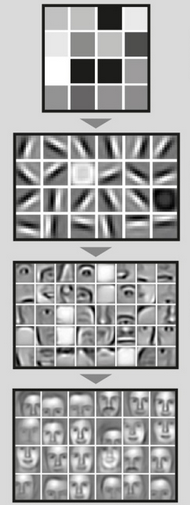
\includegraphics[height=6cm]{cnn.png}
        \caption{CNN}
        \label{fig:cnn}
    \end{subfigure}

    \caption{Comparison of object recognition hierarchies in (a) the human
    visual cortex and (b) a convolutional deep neural network. Processing
    complexity increases as layers become deeper in both models. Photo credit:
    (a) \cite{gazzaniga09}, (b) \cite{ufldl}.}
    \label{fig:comparison}
\end{figure*}

\subsection{Learning style}

Similarly to how content representations are learned by CNNs, Gatys et al.
discovered that CNNs can learn representations of style by
examining certain ``stylistic layers'' in the network. The key discovery of the
paper is that these representations are separable; that is, modifications to an
image can change the responses in the stylistic and content layers relatively
independently. This results in interesting potential for optimization, whereby
the style and content of two distinct images are combined.
 This results in interesting potential for optimization, whereby the style and
 content of two distinct images are combined.
\section{Methods}

We use the VGG-19 Deep Convolutional Neural Network \cite{Simonyan14c} trained for stylistic
representations by researchers at the Max Planck Institute for Biological
Cybernetics \cite{gatys15}. Using this model with the Caffe deep
learning framework \cite{jia14}, we extract high level representations of style
and content by capturing the response of predetermined layers in the network.

\subsection{Loss function}

Using these stylistic features Gladys et al. create a loss function that jointly
takes into account the stylistic distance from the candidate image to the style
image and the content distance from the candidate image to the content image.
By jointly minimizing this function, the style of the candidate image is
transformed while still attempting to maintain as much of the content
representation as possible, leading to a stylistically transformed image. If
$\vec{c}$ is the content image, $\vec{s}$ is the style image, and $\vec{n}$ is
the candidate image, the loss function is

\begin{equation}
  \mathcal{L}_{total}(\vec{n}, \vec{c}, \vec{s}) = \alpha \mathcal{L}_{content}
  (\vec{n}, \vec{c}) + \beta \mathcal{L}_{style}(\vec{n}, \vec{s}),
\end{equation}

where $\alpha$ and $\beta$ are configurable parameters specifying the relative
emphasis placed on the content and the style differences of the candidate
image, respectively. In our implementation, $\alpha$ and $\beta$ are encoded as
one configurable style/content ratio.

The derivative of this loss function provides us with an indication of the
direction to modify the image so that the loss function is most minimized.

\subsection{Gradient Descent}

Using these two metrics, we use a first-order optimization
technique known as gradient descent (specifically, L-BFGS) to minimize the differences between the
filter responses of the content and style images and that of the image we are creating
This is achieved by modifying the image by the
negative direction of the filter gradient magnitude, which allows us to quickly
approach a local minimum of the loss function.

Using the above procedure, we capture higher level representations of the
style of the style image and the content of the content image, initialize a new
white noise image, and perform
gradient descent to minimize the previously discussed loss function.
After an adequate number of iterations (empirically determined to be around
300), this procedure produces an image that the CNN hidden layers
determine to have style similar to that of the style target image and content
similar to that of the content target image.

\subsection{Implementational Details}

The original VGG-19 network was released to the public using the C++ deep
learning framework Caffe \cite{jia14}, so we decided to use Caffe's native
Python bindings to implement our algorithm, as both of us were familiar with
Python. In addition to the Pycaffe bindings, additional libraries used to
handle numerical computation were Scipy for optimization and matrix
multiplication (\texttt{scipy.optimize.fmin\_l\_bfgs\_b,
scipy.linalg.blas.sgemm}) and Skimage for image processing. Jupyter notebook
was used to display results from our rented server.

Because the deep learning methods used in this paper and similar tasks are very
computationally intensive, we used a GPU-specialized Amazon AWS EC2 instance
(g2.2xlarge) with Nvidia CUDA and CuDNN deep learning libraries to provide computational power for this project. Running a single
forward pass of the network on an input image took around 45 seconds on an
average Intel laptop; when computing on a server with Nvidia CUDA and CuDNN,
the same forward pass takes less than one second. This enabled us to iterate
rapidly, debugging and testing new configurations of variables to create the
optimal algorithm implementation.

\subsection{Parameter Tuning}

We made several parameters configurable, including settings for image width,
number of iterations, stylistic content weighting, and resize parameters. These
are detailed in the Appendix and discussed in the results.

\subsection{Extending the algorithm: whole-artist replication}

We attempted to extend the original algorithm by creating a program that
replicated an image not just in the style of one artist's painting (e.g.\
``Starry Night''), but rather attempted to imitate how an artist would paint an
arbitrary image. There were two obstacles we attempted to overcome.

\paragraph{Stochastic artist model}

Attempts to train gradient descent on the arithmetic mean of multiple
stylistic target images resulted in meaningless images
(Figure~\ref{fig:picasso}). We hypothesize this is because interesting feature
details in each image get averaged out. Additionally, the optimized image does
not reflect a global average, but rather, parts of the image reach local optima
as they become close to one specific stylistic image, as visible in the figure
below.

\begin{figure}[h]
  \centering
  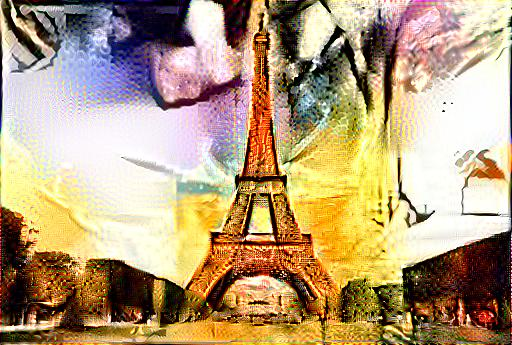
\includegraphics[width=0.8\linewidth]{picasso.jpg}
  \caption{Result of optimizing according to the stylistic mean of 45 of
  Picasso's cubist works (Still Life with the Caned Chair, Guernica, etc.)}
  \label{fig:picasso}
\end{figure}

A workaround we devised was to
 create stylistic representations of an artist based on randomly selecting a
 single artwork from that corpus.
 To obtain the necessary
quantity of artwork, we built an algorithm to scrape Wikiart for all of one artist's
paintings. We then create an image that serves as an adequate representation of
an artist's style for the particular content we are modifying by randomly
selecting an image in the body of work by that artist, and running that new
image through the network. This representation is then used in the gradient
descent process previously described.

\paragraph{Color transfer}

Color was tightly correlated with our stylistic
features; regardless of the original color of the content image, training it on
a heavily colored image such as Starry Night overwhelmingly skewed the final
image towards the color of the style image (see Figure~\ref{fig:iter}).
In order to circumvent this and obtain a more natural stylistic transfer,
regardless of color, we used a color transfer algorithm \cite{reinhard2001color} to
map the color from the content target image to the style target image prior to
generating higher level style representations with the convolutional neural
network. This resulted in stylistic representations which had colors similar to
that of the content image.

\section{Results}

Results were good and reflected the high-quality images described in the
original paper. We tried various combinations of images and paintings, and
found good results applying various paintings to a publicly available image of
the Eiffel Tower; those results are shown in Figure~\ref{fig:eiffel}. What's
more, by using the aforementioned computer architecture, we were able to
achieve good runtimes; 200 iterations of gradient descent on a final 512 px
width image generally took only around 10 minutes on our EC2 instance.

\subsection{Parameter Tuning}

\paragraph{Gradient descent iterations}

We found that gradient descent on content images showed diminishing perceptual
quality returns. The first 40 or so iterations were the biggest contributors to
the overall quality of the image; after that, 100--150 iterations showed good
strengthening of the texture of the image, removing more microscopic details
and overall participating in the ``smoothing'' of the image. Examining
differences in single iterations in the 150+ range show almost no perceptual
difference, but it is possible to see further mild improvements when making
jumps from 150 to 300+ iterations. The default convergence parameter in scipy's
L-BFGS algorithm resulted in most images converging after 600 or 700
iterations; results at this level were not visibly different than results
obtained at 300 iterations. See Figure~\ref{fig:iter} for a demonstration of
the effect of the number of iterations on image quality.

\paragraph{Style/content ratio}

The optimal style/content ratio depended on the specific image. We found that
weights of 100 ($\alpha = 1, \beta = 100$) or 1000 ($\alpha = 1, \beta = 1000$)
in favor of the stylistic loss function worked well for most images.

\paragraph{Style image resize}

The style image resize parameter depends on the size of the image to be
produced. One limitation of this algorithm is that it is not invariant to
various resolutions of style and content images. Figure~\ref{fig:stylescale}
shows the effect of scaling the stylistic image and producing an
identically-sized content image; larger scaling captures more microscopic,
texture-specific features, while smaller scaling captures more macroscopic
features. In the case of Starry Night, more overall curvature in brushstrokes
is seen with the 1.2x style scaling versus the 1.8x style scaling. As the image
to be produced increases in resolution, the stylistic image should change also
to keep the level of detail acquired similar.

\begin{figure}[h]
  \centering
  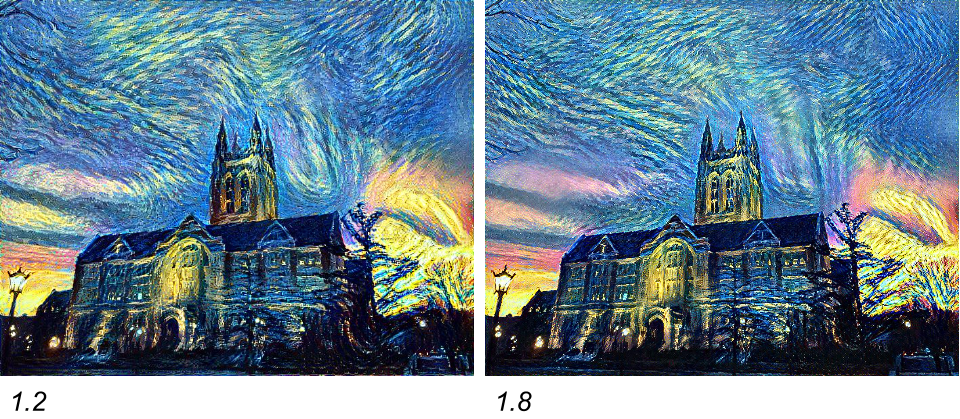
\includegraphics[width=\linewidth]{stylescale.png}
  \caption{Effect of scaling the stylistic image by 1.2x and 1.8x,
  respectively, on the stylistic content of the identically-sized output image.}
  \label{fig:stylescale}
\end{figure}

\begin{figure*}[h]
  \centering
  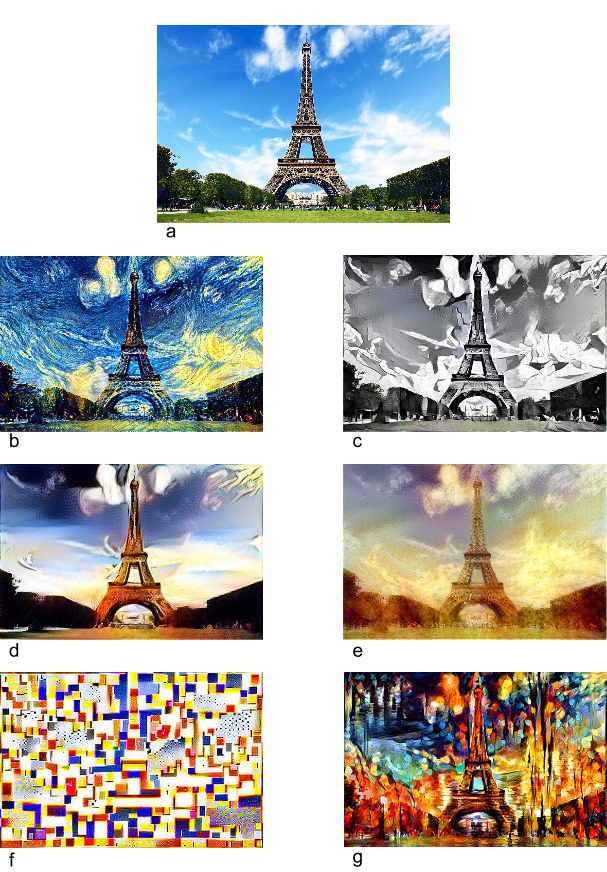
\includegraphics[width=0.8\linewidth]{eiffel.png}
  \caption{Result of applying several paintings to an image of the eiffel
  tower. Original image shown at top (a). Then, applied paintings are (b)  The
  Starry Night, Vincent Van Gogh; (c) Guernica, Pablo Picasso; (d) The
  Persistence of Memory, Salvador Dal\`i; (e) Rain, Steam, and Speed, JMW
  Turner; (f) Broadway Boogie-Woogie, Piet Mondrian; (g) Farewell to Anger,
  ieonid Afremov.}
  \label{fig:eiffel}
\end{figure*}

\begin{figure}[t]
  \centering
  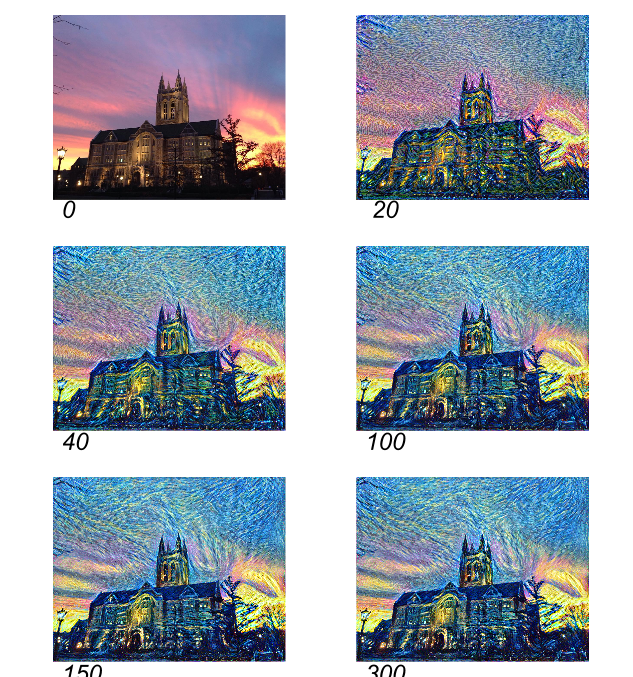
\includegraphics[width=\linewidth]{iter.png}
  \caption{Progress of numerous iterations of L-BFGS gradient descent on an
  image of Gasson Hall at Boston College in Chestnut Hill, MA. Candidate image
was initialized as the original image.}
  \label{fig:iter}
\end{figure}

\subsection{Extensions}

Our application of a color transfer algorithm worked well for some images but
was rather weaker for others. The best results produced by the color transfer
algorithm worked on stylistic images that had relatively mild coloring, so the
color of the content image was able to dominate the color of the stylistic
image. An example of using color transfer to keep the color of the content
target image is illustrated in Figure~\ref{fig:ct}.

\begin{figure}[h]
  \centering
  \includegraphics[width=\linewidth]{colortransfer.png}
  \caption{Example of applying color transfer from a nighttime picture of the
    Toronto skyline to Seurat's \emph{The Seine and la Grande Jette -
    Springtime}. }
  \label{fig:ct}
\end{figure}

\section{Conclusion}

The project provided us with a platform on which to investigate deep learning
and its potential uses in computer vision. While we were able to successfully
recreate the algorithm laid out in Gatys et al \cite{gatys15},
our initial attempts at creating a stylistic representation left much to be
desired. This led us to take look at the problem from a less technical
perspective and realize that it may be adequate to simply randomly select the
work form the artist and use that as a stylistic reference.  Additionally, we
encountered significant difficult separating texture and large scale features
from color. We managed to find a partial solution to this problem by mapping
the color space from the target content image to the target style image prior
to building the higher-level representations with the network but this often
produced substandard results and is certainly in need of improvement. A natural
next step for this project is to address the color representation by attempting
to build our target representations in HSV color space, which inherently
separates texture from color (Figure~\ref{fig:spaces}).

\begin{figure*}[t]

  \savebox{\largestimage}{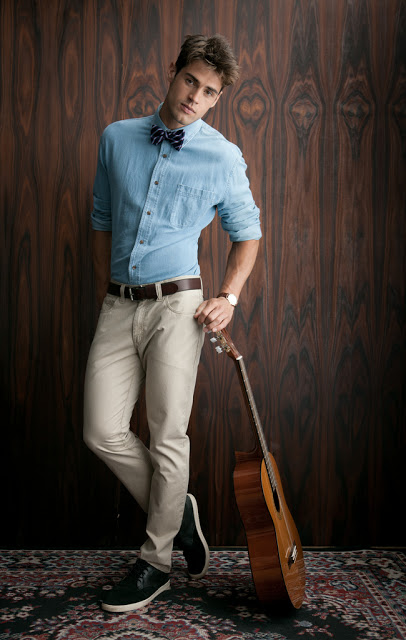
\includegraphics[width=0.3\linewidth]{ChadWhite-color.jpg}}
  \begin{subfigure}[t]{0.3\linewidth}
  \centering
        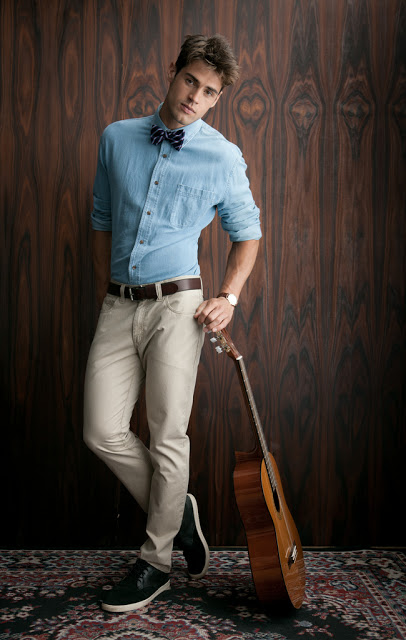
\includegraphics[height=6cm]{ChadWhite-color.jpg}
        \caption{Original}
        \label{fig:color}
  \end{subfigure}
  \quad
  \begin{subfigure}[t]{0.3\linewidth}
          \centering
          % Adjust vertical eight of smaller image
            % \raisebox{\dimexpr.5\ht\largestimage-.5\height}{%
              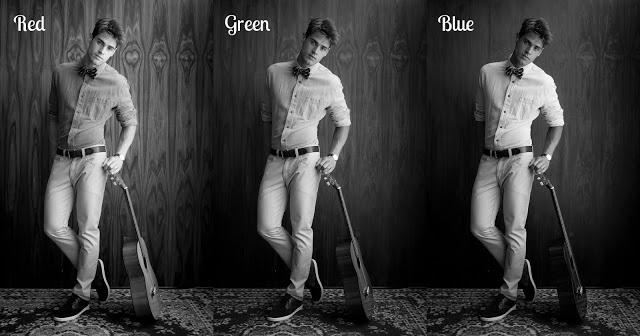
\includegraphics[height=2.5cm]{ChadWhite-RGB.jpg}
        \caption{RGB Channels}
          \label{fig:rgb}
  \end{subfigure}
  \quad
  \begin{subfigure}[t]{0.3\linewidth}
          \centering
          % Adjust vertical eight of smaller image
            % \raisebox{\dimexpr.5\ht\largestimage-.5\height}{%
              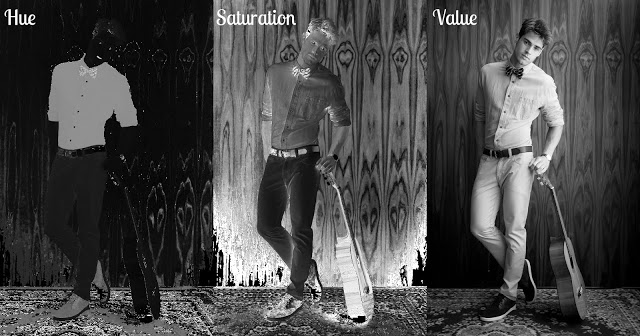
\includegraphics[height=2.5cm]{ChadWhite-HSV.jpg}
        \caption{HSV Channels}
          \label{fig:hsv}
  \end{subfigure}
  \caption{Comparison of original image with information in the images' RGB and HSV spaces.}
  \label{fig:spaces}
\end{figure*}

However it is likely that this will
challenge the convolutional neural network's ability to build reasonable
higher-level representations of images because the network was trained to
accept input images in the RGB color space.  After having completed the initial
phase of this project, we believe the most important step moving forward will be
to gain a better understanding of the convolutional neural network we are using
by running gradient descent on one layer at a time to see what it is capturing.
Up until this point, we have been treating the network as a black box that is
simply feeding it images and capturing the response of predetermined layers. In
order to extend this work in any meaningful way it has become clear that
understanding the network on a deeper level will be key.

Lastly, this project demonstrated the potential of deep learning in concrete
terms that is widely accessible to those outside of computer science,
especially in the liberal arts tradition of Boston College. This proved
incredibly rewarding as it allowed us to encourage our friends, family, and
general community to learn more about Artificial Intelligence and how it
impacts their life.

% We plan on creating a command-line tool in Python, interfacing with the Caffe
% \cite{jia14} deep learning framework via pycaffe, to first recreate the
% algorithm demonstrated in the paper and then enable support for artist
% replication. Open source implementations of the algorithm using Lua and Torch
% do exist\footnote{e.g.\
  % \href{https://github.com/jcjohnson/neural-style}{https://github.com/jcjohnson/neural-style}}
  % but we'll be building an original implementation in Python to gain a better
  % understanding of how the system works.

  % Once base functionality is
  % established, we plan on expanding upon the original algorithm in the paper by
  % attempting to recreate images not in the style of a single famous painting
  % but by the style of an artist oeuvre. This will require either 1) learning a
  % stylistic representation of an artist's lifetime work by training a network
  % on not just one, but many paintings, or 2) stochastically chosing a painting
  % or set of paintings on which to recreate a picture. Art for given artists
  % will be obtained via automated scraping of
  % WikiArt\footnote{\href{http://www.wikiart.org/}{http://www.wikiart.org/}}, which provides a large database of
  % artwork categorized by artist.

% \paragraph{Milestone 1 (10/29)} Establish GitHub repository with writeups, background
% information, and utility scripts. Create a Linux server set
% up on the Caffe and pycaffe framework, from which we will do more intensive
% computation. Download the VGG-19 Caffe model used in \cite{gatys15}. Write
% utility script to scrape artwork from WikiArt, and download art for one or two
% preliminary artists. (Done)
% \paragraph{Milestone 2 (11/12)} Develop command line tool implementing base
% functionality as described in the paper: recreating an image based
% on the style of a single image.
% \paragraph{Milestone 3 (12/3)} Enhanced functionality: develop support for
% recreating an image based on preconfigured artist style representations. For
% now we'll pick a couple of well known artists such as Van Gogh and Picasso.
% Polish and finalize CLI tool.

% \section{Deliverables}
% Deliverables include a GitHub repository of all of the work we'll complete this
% semester, including a pdf writeup of the steps taken in implementing our
% system, the Python and Caffe code, and instructions and examples.

% \section{Helpful topics from the AI course}

% \begin{itemize}
    % \item Machine learning, and specifically artificial neural networks. We will be
    % building particularly advanced models of ANNs to handle image processing
    % tasks. In learning more about deep learning, a survey by LeCun, Bengio, and
    % Hinton \cite{lecun2015}, and a review of representation learning by Bengio
    % et al. \cite{bengio2012} will be helpful.
    % \item Probability can be used to incorporate random elements into the
      % processing of the images (e.g.\ controlling style versus content
      % tradeoffs, perhaps randomly selecting paintings)
% \end{itemize}


% \section{Challenges}

% \begin{itemize}
    % \item The principal challenge is not only understanding the paper's
      % algorithm, but extending it to incorporate the stylistic content of a
      % complete body of images. From a technical perspective, this involves
      % training the CNN in charge of handling style with many images of a single
      % artist, which will also require a fundamental understanding of how the
      % network works.
    % \item Conceptually, it's unclear whether the stylistic information derived
      % from training the network on several images will result in a general
      % sense of an artist's style, or a confusing and meaningless average of an
      % artist's work. For example, some artists vary in style considerably over
      % their careers. If the latter, we need to make decisions about
      % how to obtain a sensible stylistic representation. It may be useful to
      % limit the training images to a specific subset of similar paintings.
    % \item One challenge will be optimizing computation time. CNNs are
      % computationally intensive and can take significant time to train.
      % Optimizations on both the software level, such as saving model
      % parameters, and the hardware level, such as enabling CUDA GPU
      % computation, must be taken into account when designing our system.
% \end{itemize}

\bibliographystyle{IEEEtranN}
\bibliography{final}

\clearpage

\onecolumn
\appendix[Output of \texttt{art.py} help]
\begin{verbatim}
usage: art.py [-h] [-A ARTIST] [-n NUMITER] [-w WIDTH] [-i {rand,content}]
              [-p PRINT_RATE] [-s STYLE_SCALE] [-c--color-transfer]
              content_image style_images [style_images ...]

positional arguments:
  content_image         Content image
  style_images          Style image(s)

optional arguments:
  -h, --help            show this help message and exit
  -A ARTIST, --artist ARTIST
                        Artist to imitate, Script will randomly choose an
                        artwork from this artist. Artist's work must be saved
                        in wikiart/artist_name!
  -n NUMITER, --numiter NUMITER
                        Number of iterations
  -w WIDTH, --width WIDTH
                        Max image width
  -i {rand,content}, --init {rand,content}
                        Initialize image from noise (rand) or original image
  -p PRINT_RATE, --print_rate PRINT_RATE
                        How often to save intermediate images
  -s STYLE_SCALE, --style_scale STYLE_SCALE
                        Resize style image - changes resolution of features
  -c--color-transfer    Apply color transfer algorithm to attempt to change
                        style image to match color of the content image.
\end{verbatim}

\end{document}
